\notechapter{N-20260306}{Multivariable Limits, Continuity, Differentiability, and the Total Derivative}


\section{Limits in several variables}

The statement $\lim_{(x,y)\to(x_0,y_0)}f(x,y)=A$ means that $f$ approaches $A$ along every possible approach to the point.  Checking only the two coordinate axes is not enough.  One either proves a uniform estimate in terms of $r=\sqrt{(x-x_0)^2+(y-y_0)^2}$, or disproves the limit by giving two paths with different limiting values.

\section{Continuity and partial derivatives}

Continuity at $P_0$ means
\[
  \lim_{P\to P_0}f(P)=f(P_0).
\]
The partial derivatives are
\[
\begin{aligned}
  f_x(x_0,y_0)&=\lim_{h\to0}\frac{f(x_0+h,y_0)-f(x_0,y_0)}h,\\
  f_y(x_0,y_0)&=\lim_{h\to0}\frac{f(x_0,y_0+h)-f(x_0,y_0)}h.
\end{aligned}
\]
They measure coordinate-direction changes.  Their existence alone does not imply continuity or differentiability.

\section{Differentiability as linear approximation}

The correct multivariable analogue of differentiability is the existence of a linear approximation:
\[
  f(P_0+h)=f(P_0)+L(h)+o(\|h\|).
\]
For scalar-valued $f$, the linear map is $L(h)=\nabla f(P_0)\cdot h$.  For $F:\mathbb R^n\to\mathbb R^m$, the derivative is the Jacobian matrix
\[
  DF(P_0)=\left(\frac{\partial F_i}{\partial x_j}(P_0)\right).
\]

\section{Directional derivatives and tangent planes}

For a unit vector $u$,
\[
  D_uf(P_0)=\lim_{t\to0}\frac{f(P_0+tu)-f(P_0)}t.
\]
If $f$ is differentiable, then $D_uf(P_0)=\nabla f(P_0)\cdot u$.  For a surface $z=f(x,y)$, the tangent plane is
\[
  z-z_0=f_x(x_0,y_0)(x-x_0)+f_y(x_0,y_0)(y-y_0).
\]
For $F(x,y,z)=0$, the tangent plane is $\nabla F(P_0)\cdot(P-P_0)=0$.




\section{Mixed partial derivatives as surface twist}

For a surface \(z=f(x,y)\), the mixed partial derivative
\[
  f_{xy}=\partial_x(\partial_y f)
\]
can be read geometrically as follows: first look at the slope of the \(y\)-direction tangent line, then ask how that slope changes as one moves in the \(x\)-direction.  Thus it measures a kind of local twisting of the surface rather than a new independent coordinate slope.

\begin{figure}[H]
\centering
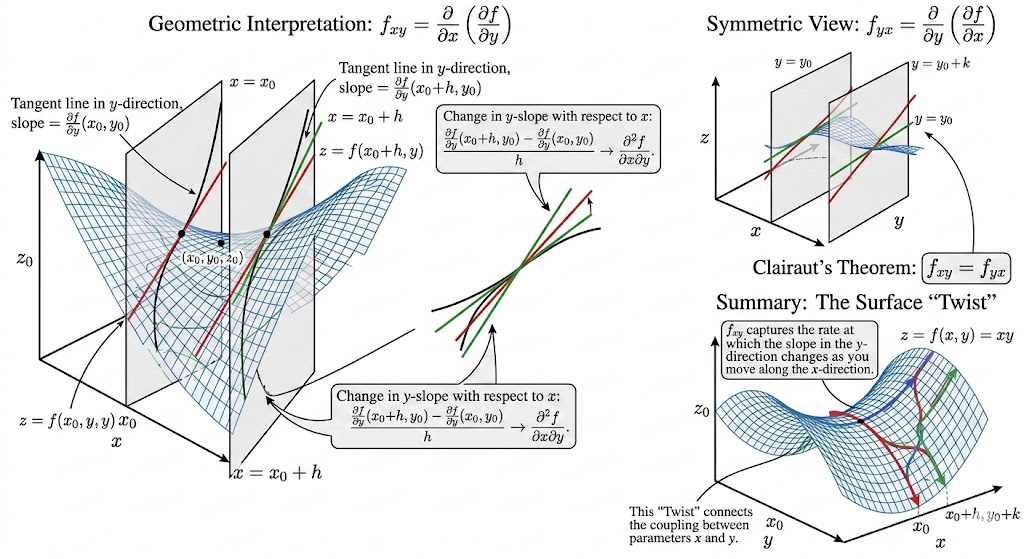
\includegraphics[width=0.94\textwidth,height=0.74\textheight,keepaspectratio]{figures/notes-md/N-20260306/N-20260306-fig-02-mixed-partial-derivative-geometric-interpretation.jpg}
\caption{Geometric interpretation of the mixed partial derivative: it measures how the \(y\)-direction slope changes as one moves in the \(x\)-direction, and symmetrically for \(f_{yx}\).}
\end{figure}

Under the usual smoothness hypotheses, Clairaut's theorem identifies the two orders:
\[
  f_{xy}=f_{yx}.
\]

\section{Expanded synthesis and advanced context}

Multivariable calculus replaces the slope of a line by a linear map.  Partial derivatives are its coordinate entries; the gradient is its vector representation in the scalar-valued case; the Jacobian is its matrix representation in the vector-valued case.



\paragraph{Expanded synthesis.}
For this chapter, the elementary material should be read as a study of what remains invariant when coordinates change. The earlier sections (`Limits in several variables`, `Continuity and partial derivatives`, `Differentiability as linear approximation`, `Directional derivatives and tangent planes`) compute with arrays, bases, pivots, determinants, or eigenvectors; the deeper object is a linear map together with the spaces it acts on. A matrix is a representation of that map after bases have been chosen. This is why formulas such as
\[
  A' = P^{-1}AP,\qquad \widetilde A = T^{-1}AS
\]
are not cosmetic: they distinguish an intrinsic morphism from a coordinate description.

The structural hierarchy is as follows. Kernels record what a map forgets, images record what it reaches, cokernels record obstructions to solvability, and quotients record information after an equivalence has been imposed. Determinants act on the top exterior power and therefore measure oriented volume; traces are invariant under cyclic rearrangement and become characters in representation theory; adjoints depend on an inner product and lead to self-adjoint spectral theory.

A useful way to return to the computations is to ask, for every formula, which invariant it is measuring. Row reduction measures rank and kernel; diagonalization measures decomposition into invariant subspaces; Gram--Schmidt measures orthogonal projection; positive definiteness measures ellipsoid geometry; tensor notation measures how components transform. The elementary methods are therefore the finite-dimensional laboratory in which duality, quotienting, functoriality, and spectral decomposition can be seen clearly.


\section{Expanded examples: why partial derivatives are not enough}

A standard counterexample is
\[
  f(x,y)=
  \begin{cases}
  \dfrac{xy}{x^2+y^2},&(x,y)\ne(0,0),\\
  0,&(x,y)=(0,0).
  \end{cases}
\]
Along the $x$-axis and $y$-axis the function is $0$, but along $y=x$ it tends to $1/2$.  Therefore the two-variable limit does not exist.

Another useful example is
\[
  f(x,y)=
  \begin{cases}
  \dfrac{x^2y}{x^4+y^2},&(x,y)\ne(0,0),\\
  0,&(x,y)=(0,0).
  \end{cases}
\]
Along every straight line $y=mx$ the limit is $0$, but along $y=x^2$ the limit is $1/2$.  This explains why checking only lines is not enough.

\section{Differentiability hierarchy}

The safe hierarchy is
\[
  C^1\Longrightarrow\text{differentiable}\Longrightarrow\text{continuous}.
\]
Existence of partial derivatives sits outside this chain unless additional hypotheses are imposed.  If the partial derivatives exist in a neighborhood and are continuous at the point, then the function is differentiable there.

\section{Frechet derivative viewpoint}

For $F:\mathbb R^n\to\mathbb R^m$, differentiability at $a$ means there is a linear map $L$ such that
\[
  \lim_{h\to0}\frac{|F(a+h)-F(a)-Lh|}{|h|}=0.
\]
The Jacobian matrix is merely the coordinate representation of $L$.  This formulation is the one that generalizes to Banach spaces.
